\chapter{Konzept}\label{concept}
Mit den zuvor behandelten Grundlagen und den Inspirationen aus Kapitel~\ref{related} wird nun ein Konzept zur Bearbeitung der Problemstellungen der in Kapitel~\ref{scenarios} definierten Fallstudien und Szenarien vorgestellt.
Grob teilt sich das Vorgehen in drei Phasen:
Falls noch kein Modell des geplanten Gebäudes vorliegt, muss dieses mithilfe eines Konstruktionsplaners erstellt werden.
Abschnitt~\ref{concept:modellierung} beschäftigt sich mit verschiedenen Möglichkeiten diesen Modellierungsvorgang zu vereinfachen.
Im Anschluss folgen einige Konzepte und Definitionen, die für das \textit{Wall Detailing} relevant sind, das die zweite Phase darstellt und in Abschnitt~\ref{concept:wall_detailing} konkretisiert wird.
Die dritte Phase beschäftigt sich damit, das Ergebnis des \textit{Wall Detailings} durch Anwenden von Regelsets in eine geordnete Form zu gießen.
Dies wird ab Abschnitt~\ref{concept:regelbasierte_bauplandeduktion} behandelt.

\section{Modellierung}\label{concept:modellierung}
Für gewöhnlich sind beim Planungsprozess eines Gebäudes oder anderer Infrastruktur eine Vielzahl an Experten aus unterschiedlichen Disziplinen beteiligt.
Ein Ziel dieser Arbeit ist es allerdings eine intuitive Konstruktionsplanung zu ermöglichen, sodass eine Einzelperson mit relativ geringer Einlern- und Modellierungszeit in der Lage ist ein Gebäude zu entwerfen.
Dieser Entwurf muss dennoch alle notwendigen Informationen für die anschließende Bauplandeduktion enthalten, ohne dass das Einpflegen dieser Daten spezielles Fachwissen voraussetzt.

Oftmals lässt sich die Komplexität einer Sache oder eines Vorgehens durch die Vorgabe von Einschränkungen reduzieren.
Dabei ist es allerdings wichtig diese Einschränkungen so zu wählen, dass die damit erzielten Ergebnisse nach wie vor von Nutzen sind.

\subsection{Raster}\label{concept:raster}
Im Fall von Gebäude- oder besser Gebilde-Konstruktionen existieren bereits einige Beispiele, die durch Einschränkungen so stark vereinfacht werden, dass sogar Kinder damit umgehen können.
Das wohl bekannteste ist das Lego System (siehe Kapitel~\ref{basics:lego}).
Neben dessen nützlichen Steckverbindungen, die es ermöglichen ohne Anwenden von Klebstoff oder Schrauben Steine aneinander zu befestigen, ist für diese Arbeit das dadurch vorgegebene Raster ein interessantes Konzept zur Vereinfachung der Modellierung von Gebäuden.
In Kapitel~\ref{basics:Mauerwerksbau} wurden auch schon die Begriffe \textit{Baunennmaß} und des \textit{Baurichtmaß} eingeführt und das oktametrischen Maßsystem vorgestellt.
Dies entspricht im Prinzip ebenfalls einem Raster, das aber in Realität durch die Möglichkeit des Zerschneidens von Bausteinen nicht zwingend eingehalten werden muss.
Da das Vorgeben eines Rasters, dem sowohl die Größen der zu verwendenden Bausteine, als auch (im Fall des Lego Systems) deren Platzierung folgen müssen, eine Einschränkung darstellt, die im Einklang mit der Intuition vieler Menschen steht, wurde dies in das Modellierungskonzept dieser Arbeit integriert.
Das Vorgeben eines einzigen, fest definierten Rasters stellt allerdings eine zu große Einschränkung dar, weshalb das Definieren verschiedener Rastergrößen möglich sein muss.
So können Modelle erstellt werden, die sowohl genau dem Lego System oder dem oktametrischen Maßsystem entsprechen, als auch beliebig anderen Rastern.

Die Modellierungsumgebung kann mithilfe von Rasterinformationen eines Objektes für dessen korrekte Platzierung, Skalierung und Rotation sorgen, indem eine solche Transformation auf die nächstliegende Größenordnung des Rasters gerundet wird.
Im Beispiel eines Rasters von \([1.0m, 1.0m, 1.0m]\) würde demnach ein auf \([0.9m, -0.7m, 0.1m]\) zu translatierendes Objekt an die Position \([1.0m, -1.0m, 0.0m]\) versetzt werden.
Da aber gewünschte valide Rotationen nicht aus einem derart vorgegebenen Raster interpretierbar sind, kann diese zusätzliche Information mithilfe eines kleinstmöglichen Winkelschritts angegeben werden.
In den Modellen der Fallstudien aus Kapitel~\ref{scenarios} werden zum Beispiel ausschließlich Rotationen eines Vielfachen von 90\degree{} verwendet, was neben den Rastern ebenfalls hinterlegt wurde.
Damit kann die Modellierungsumgebung auch den Rotationen von Objekten durch Runden eine Art Raster aufzwingen.

\subsection{Wandstück}
Auch die schiere Menge verschiedener Bestandteile eines Hauses ist für eine Einzelperson ohne Vorkenntnisse nicht überblickbar.
Da das Ziel dieser Arbeit das automatische Generieren von Legeplänen für Bausteine innerhalb der Wände eines Gebäudes darstellt, lässt sich diese Menge vorerst auf zwei wesentliche Objekttypen reduzieren:
Wände und Öffnungen in Wänden.
Öffnungen werden zum Beispiel für Fenster oder Türen benötigt.
Da eine Wand im Prinzip ein arbiträrer geometrischer Körper sein kann, dies abzubilden aber wieder die Komplexität der Modellierung steigert, wird deren Form auf einen beliebig skalierten Quader beschränkt.
Ein solcher Quader wird nachfolgend auch als \textit{Wandstück} bezeichnet.
Ein solches Wandstück besitzt demnach auch die Eigenschaften eines Quaders: eine Skalierung, eine Rotation um seinen eigenen Mittelpunkt und eine Translation im Raum.
Nachfolgend werden die Begriffe Länge, Breite und Höhe zur einfachen Unterscheidung von einer Skalierung in X, Y und Z Richtung verwendet.
Während Länge und Höhe dem Raster entsprechend beliebig gewählt werden können, ergibt sich die Breite aus dem gewählten Bausteinformat (auch als \textit{Modul} bezeichnet) und dem geplanten Mauerwerksverband (siehe Kapitel~\ref{basics:Mauerwerksbau}).
Der Verband und das Modul können jedem Wandstück als sogenannter \textit{Wandtyp} zugewiesen werden.
Dadurch ist es möglich, verschiedene Arten von Wänden innerhalb eines Gebäudemodells zu verwenden.
Diese Informationen werden später dafür verwendet, die durch das Wandstück abgesteckten Dimensionen sinnvoll mit Bausteinen zu füllen.

\subsection{Mauerwerksverband}\label{concept:mauerwerksverband}
In Kapitel~\ref{basics:Mauerwerksverband} wurden bereits einige verschiedene Mauerwerksverbände behandelt.
Um dem Wall Detailing Verfahren diese und beliebig andere Verbände in einer interpretierbaren Weise zur Verfügung stellen zu können, wird dafür eine mathematische Notation benötigt.
Bei genauer Betrachtung handelt es sich bei den meisten Mauerwerksverbänden um ein sich wiederholendes Muster.
Dabei wiederholen sich sowohl die Bausteintransformationen innerhalb einer Schicht des Verbandes, als auch dessen Schichten selbst.
Daher sind folgende Informationen zur Beschreibung eines Mauerwerksverbands notwendig:

\begin{enumerate}
    \item Eine Menge einzigartiger Schichten, bis diese sich (mit einem Versatz) wiederholen.
    \item Für jede Schicht eine Menge verschiedener Bausteintransformationen, bis diese sich (ebenfalls mit einem Versatz) wiederholen.
\end{enumerate}

Ein Mauerwerksverband kann damit als Menge von Schichten verstanden werden, die sich wiederum aus einer Menge von Bausteintransformationen zusammensetzen.
Diese Schichten besitzen jeweils einen festgelegten, darunter liegenden Vorgänger sowie einen darüber liegenden Nachfolger.
Das bedeutet, die Reihenfolge in der Schichten eines Mauerwerksverbands auftreten, darf nicht verändert werden.
Leicht zu sehen ist dies am Beispiel eines Kreuzverbandes, der durch Veränderung der Reihenfolge seiner Schichten, seine typische kreuzartige Form verlieren würde.

Eine Bausteintransformation wird in dieser Arbeit als Tupel mit folgendem Inhalt definiert:

\begin{enumerate}
    \item Eine skalierbare Position \(\vec{p} = {[x, y, z]}^T\).
    \item Eine skalierbare Rotation \(r = (x, y, z)\) angegeben in Euler-Winkeln.
    \item Einen festen translativen Versatz \(\vec{p}_o = {[x, y, z]}^T\).
    \item Einen festen rotierenden Versatz \(r_o = (x, y, z)\) ebenfalls in Euler-Winkeln.
\end{enumerate}

Skalierbar bedeutet in diesem Fall, dass die Werte von beispielsweise der Position eines Bausteins in Abhängigkeit eines veränderbaren Faktors stehen.
Zur endgültigen Platzierung eines Bausteins anhand einer Bausteintransformation aus einer Schicht eines Mauerwerksverbands wird lediglich noch ein Faktor benötigt, der angibt, die wievielte Wiederholung der Menge an Bausteintransformationen einer Schicht gerade Anwendung findet.
Sei \(B_1 = (\vec{p}, r, \vec{p}_o, r_o) = ({[l, 0, 0]}^T, (0, 0, 0), {[0, 0, 0]}^T, (0, 0, 0))\) eine Bausteintransformation, \(M = (l, b, h) = (2, 1, 1)\) ein Modul und \(c\in\mathbb{N}\) ein Skalar,
dann ergibt sich die Position \(P\) eines Bausteins zur Wiederholung \(c = 1\) wie folgt: \(P = \vec{p}_o + c * \vec{p} = {[0, 0, 0]}^T + 1 * {[2, 0, 0]}^T = {[2, 0, 0]}^T\).
Im nächsten Wiederholungsschritt mit \(c = 2\) ergibt dies eine Position \(P = {[4, 0, 0]}^T\).
Da die Rotationen als Euler-Winkel vorliegen, kann diese in ähnlicher Weise berechnet werden.
Sie beschreibt die Rotation um den Mittelpunkt des Bausteins.
In den meisten Fällen ist \(r\) allerdings gleich \((0, 0, 0)\) und \(r_o\) entweder ebenfalls \((0, 0, 0)\) oder \((0, 0, \frac{\pi}{2})\).
Letzteres entspricht einer festen Rotation um 90\degree{} um die z-Achse des Bausteins, unabhängig des Wiederholungsschritts \(r\).

\begin{figure}[hb!]
    \centering
    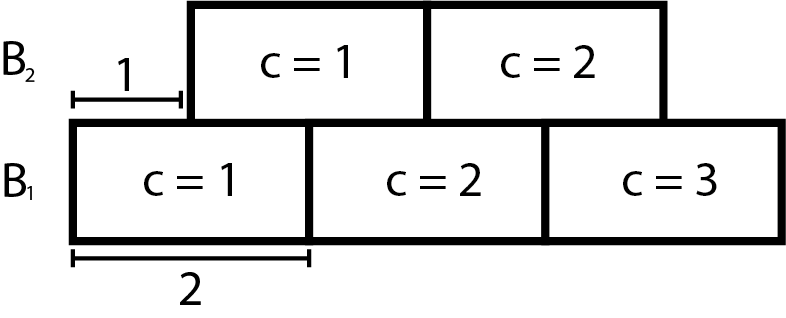
\includegraphics[width=0.7\columnwidth]{fig/concept_Mauerwerksverband.png}
    \caption{Der Läuferverband mit einem Versatz von 50 \%.}\label{fig:concept:concept_Mauerwerksverband}
\end{figure}

Mit \(B_2 = ({[l, 0, 0]}^T, (0, 0, 0), {[\frac{l}{2}, 0, 0]}^T, (0, 0, 0))\) und je einer Schicht gebildet aus den Mengen \(\{B_1\}\) bzw. \(\{B_2\}\) erhält man bereits eine komplette Beschreibung für den Läuferverband mit einem Versatz von 50 \% der Steinlänge.
Dieses Beispiel ist in Abbildung~\ref{fig:concept:concept_Mauerwerksverband} schematisch dargestellt.
Aber auch andere, komplexere Verbände können in dieser Form abgebildet und so dem nachfolgenden Wall Detailing in abstrahierter Weise übergeben werden.

\begin{figure}[ht!]
    \centering
    \begin{subfigure}[b]{0.3\columnwidth}
      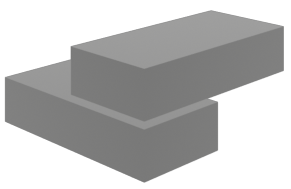
\includegraphics[width=\columnwidth]{fig/concept_streched_bond_corner.png}
      \caption{Erst \(E_1\), dann \(E_2\).}\label{fig:concept:concept_streched_bond_corner}
    \end{subfigure}
    \hfil
    \begin{subfigure}[b]{0.3\columnwidth}
      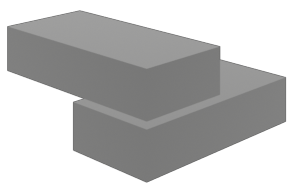
\includegraphics[width=\columnwidth]{fig/concept_streched_bond_corner_inverse.png}
      \caption{Erst \(E_2\), dann \(E_1\).}\label{fig:concept:concept_streched_bond_corner_inverse}
    \end{subfigure}
    \hfil
  \caption{Eckpläne für den Läuferverband mit einem Versatz von 50\%.}\label{fig:concept:corner_bond}
\end{figure}

Die speziellen Legepläne zur korrekten Auflösung von kritischen Bereichen wie zum Beispiel Ecken können ebenfalls in dieser Form für jeden Mauerwerksverband angegeben werden.
Für das vorangegangene Beispiel sähe der Eckplan wie folgt aus:
Eine Nulltransformation \(E_1 = ({[0, 0, 0]}^T, (0, 0, 0), {[0, 0, 0]}^T, (0, 0, 0))\) in der ersten Schicht und eine Bausteintransformationen 
\(E_2 = ({[0, 0, 0]}^T, (0, 0, 0), {[0, 0, 0]}^T, (0, 0, \frac{\pi}{2}))\) mit einer festen 90\degree{} Rotation um die z-Achse in der Zweiten.
Dieser Eckplan ist in Abbildung~\ref{fig:concept:corner_bond} zu sehen.
Ein Beispiel, in welchem dieser Eckplan angewandt wird, wurde bereits in Abbildung~\ref{fig:basics:mauerwerk_eckloesung} in Kapitel~\ref{basics:Mauerwerksverband} gezeigt.
Der einzige Unterschied zwischen dem Plan eines Mauerwerksverbands für gerade Wände und dessen Spezialplänen ist deren Anwendung.
Während aus dem Eckplan später für jede Schicht nur ein Baustein pro hinterlegter Bausteintransformation erzeugt werden muss, können beliebig lange gerade Wandabschnitte mithilfe des oben angesprochenen Wiederholungsschritts mit Bausteinen aufgefüllt werden.

\subsection{Beziehungen zwischen Wandstücken}\label{concept:relations_wandtuecke}
In dieser Arbeit stehen Wandstücke zueinander in einer Beziehung, sobald sie sich berühren oder schneiden.
Diese Beziehungen sind relevant, um die gewählten Mauerwerksverbände ordnungsgemäß über mehrere voneinander abhängige Wandstücke anzuwenden, ohne dass es zu Verletzungen von Vorschriften und Normen wie etwa dem Überbindemaß aus Kapitel~\ref{basics:Mauerwerksverband} kommt.
Wie bereits in Abschnitt~\ref{basics:Mauerwerksverband} angesprochen, treten verschiedene Arten von Beziehungen auf, die für das nachfolgende \glqq{}Wall Detailing\grqq{} zu unterscheiden sind.
Zur Modellierung von Gebäuden sind vor allem folgende Beziehungen unabdingbar:
\textit{Ecken}, \textit{T-Kreuzungen} und \textit{X-Kreuzungen}.
Diese stellen wichtige Elemente bei der Planung von Gebäuden dar. 
Nur so ist es möglich abgeschlossene und aneinanderhängende Räume zu erstellen.
Eine weitere, nicht ganz offensichtliche Beziehung besteht zwischen zwei Wandstücken, die in Verlängerung zueinander stehen, also gemeinsam einen größeren Wandbereich abdecken.
Diese Beziehung wird nachfolgend \textit{Wandstückverbund} genannt.
Bei allen vier Beziehungen handelt es sich Sonderfälle, für welche sich der Mauerwerksverband nicht ohne weiteres anwenden lässt, sondern teilweise explizit vorgegebene Legepläne angewandt werden müssen.
Darum ist es notwendig diese Bereiche ausfindig zu machen und voneinander unterscheiden zu können.
Es werden nun für jede dieser Beziehungen Eigenschaften aufgezeigt anhand derer man diese in einer Menge an Wandstücken erkennen kann.

\begin{figure}[ht]
    \centering
    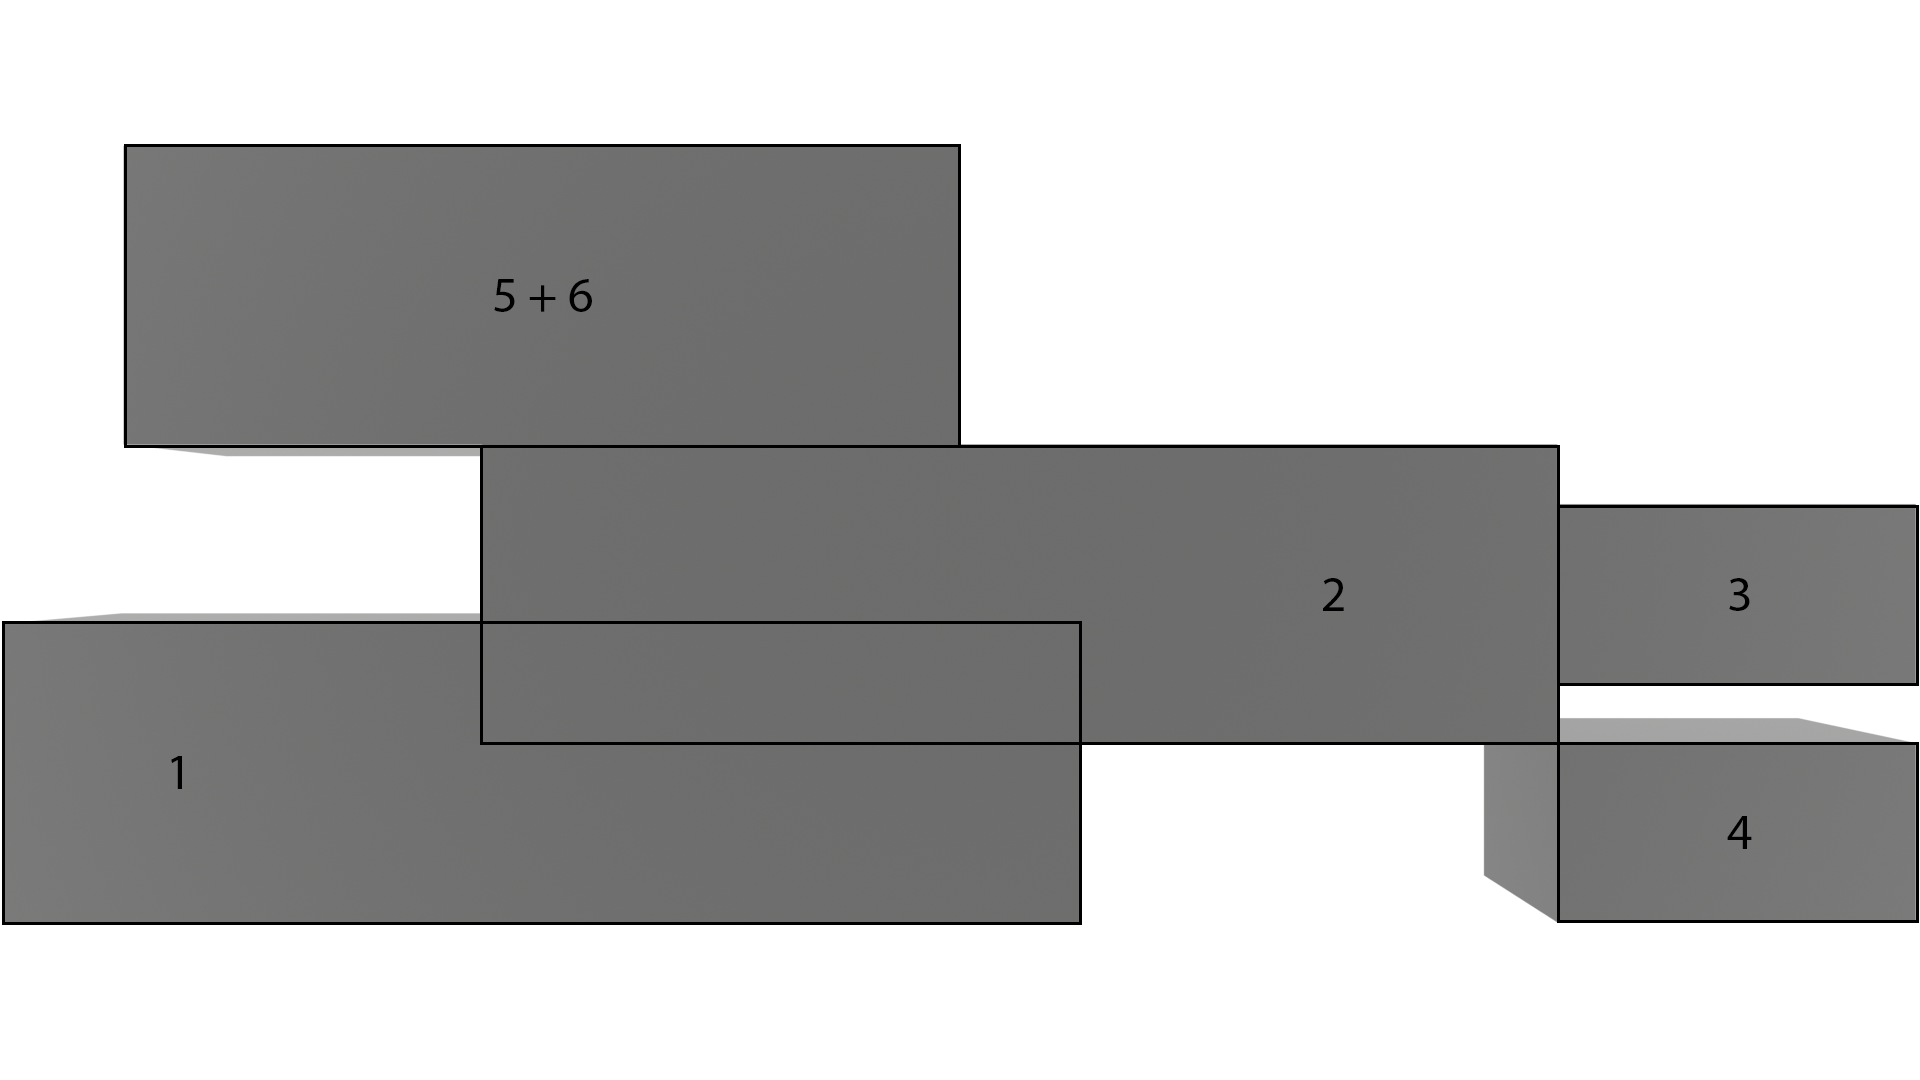
\includegraphics[width=0.8\columnwidth]{fig/Real_Combination_Base_labeled.png}
    \caption{Modell einer Wand, die durch 7 einzelne Wandstücke desselben Typs gebildet wird, deren Mittelpunkte alle auf einer Ebene liegen.}\label{fig:concept:combination_example_base}
\end{figure}

\paragraph*{Wandstückverbände}\label{concept:combination_properties} sind alle Wandstücke,  die zwar in dem Modellierungsprozess des Gebäudes durch mehrere einzelne Wandstücke realisiert wurden, eigentlich aber eine Einheit darstellen. 
Es ist notwendig alle Wandstücke zu identifizieren, die einen zusammenhängenden Wandbereich bilden, um den gewählten Mauerwerksverband korrekt über alle Wandstücke hinweg anzuwenden.
Andernfalls würde jedes Wandstück den Mauerwerksverband unabhängig seiner Nachbarn neu beginnen und ihn dadurch zwischen Wandstückübergängen häufig fälschlicherweise unterbrechen.
Ein umfangreiches Beispiel ist in Abbildung~\ref*{fig:concept:combination_example_base} dargestellt.
Um zu überprüfen, ob zwei Wandstücke eine Einheit bilden, kann das Paar auf folgende Eigenschaften getestet werden:

\begin{enumerate}
    \item Beide Wandstücke verwenden dasselbe Modul und sind während der Modellierung mit den gleichen Wandtyp annotiert worden. 
    Dies verhindert vor allem das Kombinieren unterschiedlich dicker Wände.
    \item\label{real:z_parallel} Die lokalen Z-Achsen beider Wandstücke sind parallel. 
    Dies verhindert das Kombinieren unpassend rotierter Wandstücke.
    Die Überprüfung der Parallelität der Z-Achsen beider Wandstücke wird wie folgt durchgeführt:

    Sei \(\vec{v}_z = {[0, 0, 1]}^T\)
    eine z-Achse und \(v_z = (v_w, v_x, v_y, v_z) = (0, 0, 0, 1)\) das dazugehörige Quaternion. 
    Außerdem seien \(q_1\) und \(q_2\) die beiden Rotationen der Wandstücke. Dann stellen 
    \(v_{z^1} = q_1 * v_z * q_1^{-1}\) und 
    \(v_{z^2} = q_2 * v_z * q_2^{-1}\) die jeweiligen \glqq{}Z-Anteile\grqq{} dieser Rotationen dar.
    Daraus ergeben sich die \glqq{}Z-Vektoren\grqq{} wie folgt: 
    \(\vec{v}_{z^1} = {[v_{z^1_x}, v_{z^1_y}, v_{z^1_z}]}^T\) und
    \(\vec{v}_{z^2} = {[v_{z^2_x}, v_{z^2_y}, v_{z^2_z}]}^T\).
    Ist nun \(|\vec{v}_{z^1} \cdot \vec{v}_{z^2}| = 1\) gegeben, so sind die lokalen Z-Achsen der Wandstücke gleich oder um exakt 180\degree{} verdreht und damit Parallelität erfüllt.
    \item Die lokalen X-Achsen beider Wandstücke sind ebenfalls parallel. Das Vorgehen zur Überprüfung entspricht dem von Punkt~\ref{real:z_parallel}, nur dass \(v_z\) durch \(v_x = (0, 1, 0, 0)\), also der x-Achse, ersetzt werden muss.
    \item Sie stehen auf derselben Höhe oder versetzt um ein Vielfaches der gemeinsamen Modulhöhe.
    \item\label{concept:schichten} Es liegt eine Berührung oder gar eine Überlappung vor.
\end{enumerate}

Insgesamt bilden in dem Beispiel in Abbildung~\ref{fig:concept:combination_example_base} demnach alle Wandstücke mit Ausnahme von Wandstück Nummer 4 eine Einheit, die alle obigen Eigenschaften erfüllt.
Dies sind in der Tat all die Wandstücke, die den Start des gewählten Mauerwerksverbands ihren Nachbarn entsprechend anpassen müssen, sodass sich der Verband gleichmäßig über alle Wandstücke erstreckt.

\paragraph*{Ecken, T-Kreuzungen und X-Kreuzungen}\label{concept:corner_etc_properties} stellen Beziehungen zwischen einzelnen Wandstücken oder den kombinierten Wandstückverbänden aus Abschnitt~\ref{concept:combination_properties} dar.
Wie schon zu Beginn dieses Abschnitts vorweggenommen, existieren für jeden Mauerwerksverband und je nach verwendetem Modul eigene Varianten für Eck- und Kreuzungslegepläne, an welchen sich Maurer orientieren.
Einige Beispiele hierfür wurden schon in Kapitel~\ref{fig:basics:mauerwerk_eckloesung} gegeben.
Der Grund dafür ist die Komplexität in diesen Bereichen die vorgeschriebenen Normen (wie etwa dem in Abschnitt~\ref{basics:Mauerwerksverband} genannten Überbindemaß) einzuhalten.
Diese speziellen Pläne werden dann an den notwendigen Stellen angewandt - meistens bevor ein dazwischenliegender gerader Wandabschnitt mit Bausteinen aufgefüllt wird.
Es liegt deshalb nahe, die Eck- und Kreuzungslegepläne zur Beschreibung des Mauerwerksverbands hinzuzufügen, wie es schon im Abschnitt~\ref{concept:mauerwerksverband} definiert wurde.
Durch das vorangegangene Kombinieren mehrerer Wandstücke zu einer Einheit, können nachfolgend Wandstücke auch das Ergebnis solcher Kombinationen sein, aber aufgrund deren Parallelität wie ein einzelnes behandelt werden.
Da sich Ecken, T-Kreuzungen und X-Kreuzungen stark ähneln, besitzen sie einige geteilte Eigenschaften:
\begin{enumerate}
    \item\label{concept:tmp1} Beide Wandstücke verwenden dasselbe Modul und sind während der Modellierung mit den gleichen Wandtyp annotiert worden.
    \item Die lokalen Z-Achsen beider Wandstücke sind parallel. Das Vorgehen zur Überprüfung ist dasselbe wie in Abschnitt~\ref{concept:combination_properties}.
    \item Sie stehen auf derselben Höhe oder versetzt um ein Vielfaches der gemeinsamen Modulhöhe.
    \item\label{concept:tmp4} Mindestens eines der beiden Wandstücke endet auf einem anderen.
\end{enumerate}

\begin{figure}[ht]
    \centering
    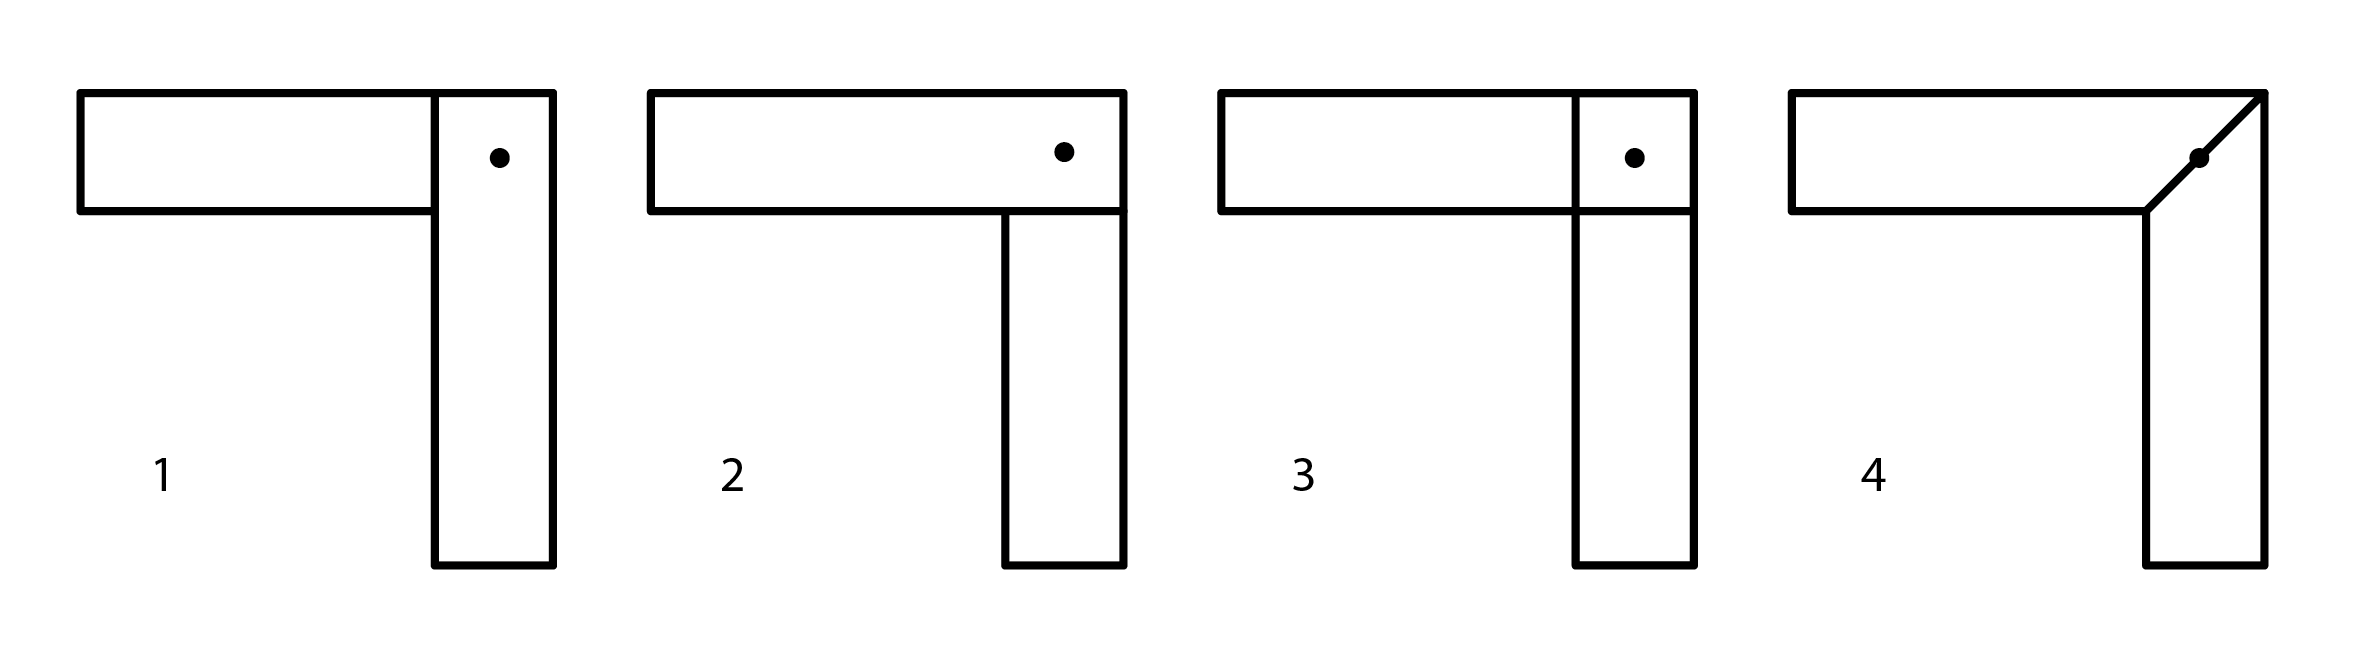
\includegraphics[width=0.8\columnwidth]{fig/ecken_variationen.png}
    \caption{Draufsicht auf Varianten der Modellierung einer Ecke.}\label{fig:concept:ecken_variationen}
\end{figure}

\begin{figure}[ht]
    \centering
    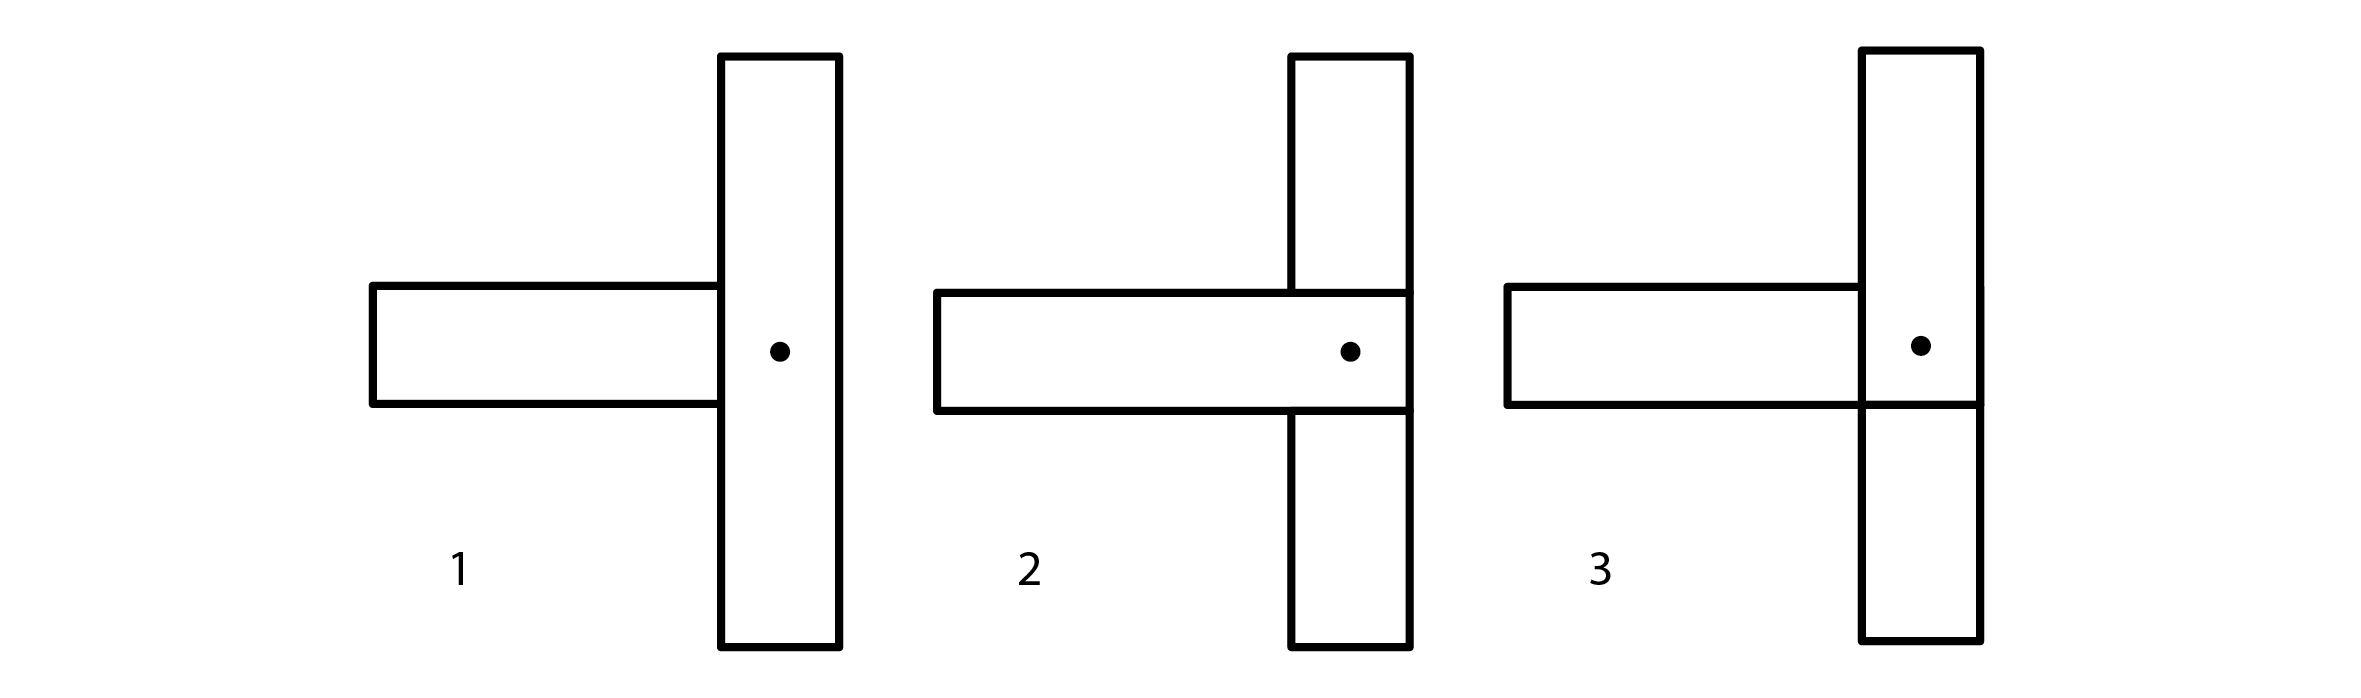
\includegraphics[width=0.8\columnwidth]{fig/t_joint_variationen.png}
    \caption{Draufsicht auf Varianten der Modellierung einer T-Kreuzung.}\label{fig:concept:t_joint_variationen}
\end{figure}

\begin{figure}[hb]
    \centering
    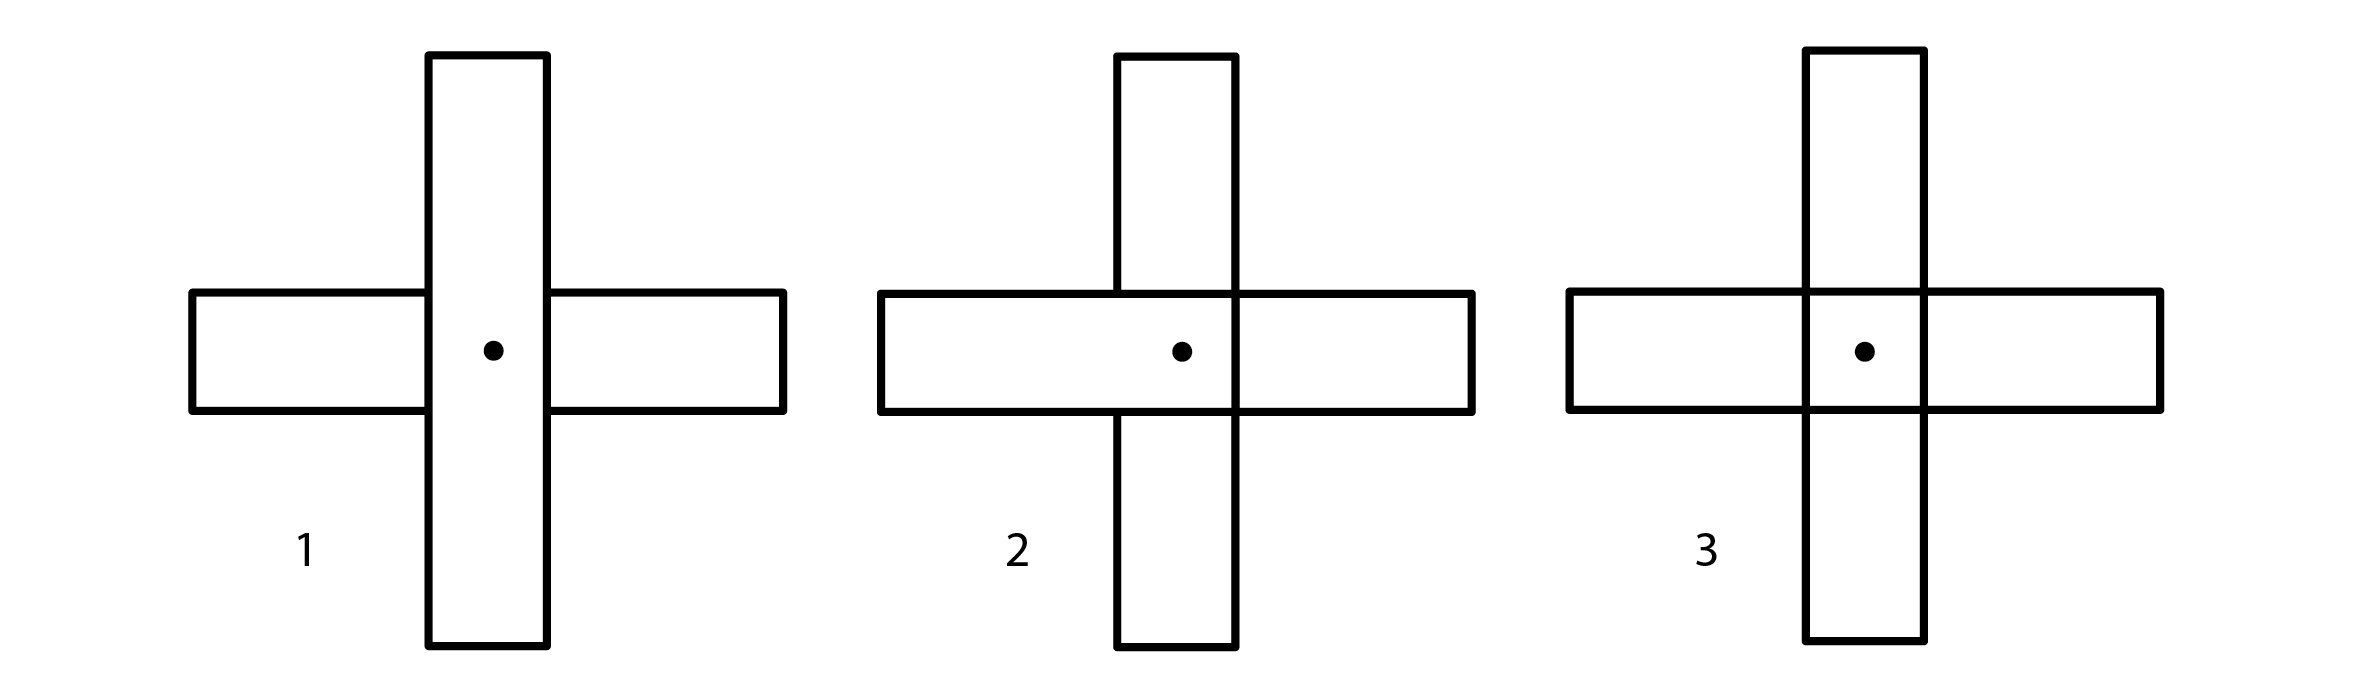
\includegraphics[width=0.8\columnwidth]{fig/x_joint_variationen.png}
    \caption{Draufsicht auf Varianten der Modellierung einer X-Kreuzung.}\label{fig:concept:x_joint_variationen}
\end{figure}

Sind diese Eigenschaften erfüllt, werden die Schnittpunkte der Richtungsvektoren entlang der lokalen X-Achsen beider Wandstücke errechnet.
Im Falle einer einfachen Ecke oder einer T-Kreuzung, existiert nur ein einzelnes Paar an Wandstücken, die sich im Mittelpunkt der Ecke oder der T-Kreuzung schneiden.
Der Unterschied ist lediglich die Stelle des Schnittpunkts relativ zu den beiden Wandstücken.
Sei \(w_1\) die Breite von einem und \(w_2\) die des anderen Wandstücks, so gilt nach Punkt~\ref{concept:tmp1} \(w_1 = w_2\).
Liegt der errechnete Schnittpunkt bei beiden Wandstücken näher als \(\frac{w_1}{2}\) entlang der lokalen x-Achse an einer der beiden Außenkanten handelt es sich um eine Ecke, da beide Wandstücke an diesem Punkt enden.
Falls der Schnittpunkt bei einem der beiden Wandstücke allerdings mindestens  \(\frac{w_1}{2}\) innerhalb des Wandstücks liegt, so handelt es sich um eine T-Kreuzung.
Ein Wandstück steht also auf einem Anderen.
Dies ist in den Abbildungen~\ref{fig:concept:ecken_variationen} und~\ref{fig:concept:t_joint_variationen} zu sehen. 
Werden für zwei unterschiedliche Paare dieselben Schnittpunkte errechnet, so kann es sich entweder um eine mit drei Wandstücken modellierte T-Kreuzung oder X-Kreuzung handeln.
Treffen sich an dem Schnittpunkt zwei Ecken, ergibt sich daraus eine T-Kreuzung (siehe Fall 2 in Abbildung~\ref{fig:concept:t_joint_variationen}).
Teilen sich aber zwei T-Kreuzungen dieselben Schnittpunkte, so sind alle Voraussetzungen für eine X-Kreuzung gegeben (siehe Fall 1 in Abbildung~\ref{fig:concept:x_joint_variationen}).
Einen Sonderfall für Punkt~\ref{concept:tmp4} stellt eine X-Kreuzung dar - modelliert aus zwei sich schneidenden Wandstücken.
Dieser Fall ist in Abbildung~\ref{fig:concept:x_joint_variationen} mit der Variante Nummer 3 dargestellt.
Hier liegt der Schnittpunkt des Wandstück-Paares mindestens \(\frac{w_1}{2}\) innerhalb beider Wandstücke und keines der Wandstücke endet auf dem Anderen.
Durch das vorhergehende Kombinieren von Wandstücken werden die Fälle 3 aus Abbildung~\ref{fig:concept:t_joint_variationen} und 2 aus Abbildung~\ref{fig:concept:x_joint_variationen} eliminiert, denn dabei erfüllen jeweils zwei Wandstücke alle Eigenschaften, um nach Abschnitt~\ref{concept:combination_properties} zu einer Einheit verschmolzen zu werden.
So entsteht aus Fall 3 aus Abbildung~\ref{fig:concept:t_joint_variationen} der Fall Nummer 1 und auch Fall Nummer 2 aus Abbildung~\ref{fig:concept:x_joint_variationen} wird zu deren 1. Fall.

\subsection{Lösen von Beziehungen}\label{concept:solving_beziehungen}
Durch Ecken, T- und X-Kreuzungen werden ansonsten unabhängige Wandstücke miteinander verkettet.
Das kann zu Situationen führen, in welchen das einfache Anwenden eines Mauerwerksverbands Lücken in manchen Wandstücken hinterlässt.
Das Beispiel in Abbildung~\ref{fig:concept:loesen_von_beziehungen1} soll helfen diese Problematik zu veranschaulichen.
Zu sehen ist eine Konstellation von vier Wandstücken, die in einer Kette durch drei Ecken miteinander verbunden sind.
Das anzuwendende Modul hat die Dimensionen \([2, 1, 0.5]\). 
Die Höhe des Moduls ist für dieses Problem allerdings irrelevant, weshalb die folgenden Skizzen ausschließlich die Draufsicht auf die Situationen zeigen.
Wie in Kapitel~\ref{concept:mauerwerksverband} am Beispiel des Läuferverbands gezeigt, gibt es mehrere Möglichkeiten einem Eckplan zu folgen.
Solange die Reihenfolge weiterhin eingehalten wird, kann mit jeder Schicht des Eckplans begonnen werden einen Eckbereich aufzufüllen.
Das führt in dem Beispiel aufgrund des zweischichtigen Eckplans des Läuferverbands dazu, dass für jede der drei Ecken zwei mögliche Startschichten existieren.
Dies resultiert demnach in insgesamt acht unterschiedlichen Varianten, von welchen allerdings nicht alle zielführend sind.
In Abbildung~\ref{fig:concept:loesen_von_beziehungen2} ist eine Variante dargestellt, die Lücken in der Wand hinterlassen würde.
Das zunächst naheliegend wirkende Füllen der Löcher durch kleinere Bausteine ist nicht zulässig, da damit das Überbindemaß (siehe Kapitel~\ref{basics:Mauerwerksverband}) verletzt wäre.
Darum ist es notwendig eine Kombination an Startschichten über alle miteinander verbundenen Eckbereiche zu finden, die es ermöglicht die verbleibenden geraden Wandstücke im Anschluss durch einfaches Anwenden des Läuferverbands aufzufüllen, ohne dass Lücken entstehen.

\begin{figure}[]
    \centering
    \includegraphics[width=0.4\columnwidth]{fig/concept lösung von beziehungen1.png}
    \caption{Draufsicht auf eine Verkettung von 4 Wandstücken durch 3 dazwischenliegende Ecken.}\label{fig:concept:loesen_von_beziehungen1}
\end{figure}

\begin{figure}[]
    \centering
    \includegraphics[width=0.4\columnwidth]{fig/concept lösung von beziehungen2.png}
    \caption{Draufsicht auf eine unzulässige Lösung der Eckplankonfiguration.}\label{fig:concept:loesen_von_beziehungen2}
\end{figure}


\begin{figure}[ht!]
    \centering
    \begin{subfigure}[b]{0.4\columnwidth}
      \includegraphics[width=\columnwidth]{fig/concept lösung von beziehungen3.png}
      \caption{Eine zulässige Lösung.}\label{fig:concept:loesen_von_beziehungen3}
    \end{subfigure}
    \hfil
    \begin{subfigure}[b]{0.4\columnwidth}
      \includegraphics[width=\columnwidth]{fig/concept lösung von beziehungen4.png}
      \caption{Die darüberliegende Schicht.}\label{fig:concept:loesen_von_beziehungen4}
    \end{subfigure}
  \caption{Eine mögliche Lösung und die durch die Eckpläne entstehende zweite Lösung für die darüber liegende Schicht.}\label{fig:concept:loesen_von_beziehungen3und4}
\end{figure}

Ein Verfahren, welches für das vorliegende Beispiel des halb versetzten Läuferverbands, dessen sehr einfachen Eckplans und dem durch seine praktische Form gewählten Moduls Lösungen findet, löst nicht zwangsläufig auch eine beliebig andere Situation.
Ebenfalls führt das Miteinbeziehen der 3. Dimension, also der Höhe der beteiligten Wandstücke, zu einer erheblichen Vervielfachung möglicher Eck-Konstellationen.
Zieht man etwa das Beispiel aus Abbildung~\ref{fig:concept:combination_example_base} heran und erweitert es durch Einfügen weiterer Wandstücke um Ecken an den Außenkanten von Bereich 1, 3, 4, 5 + 6 und 7, an welchen beliebig weitere verkettete Wandstücke in sich geschlossene Kreise bilden, so können sogar nicht lösbare Fälle auftreten.
Durch die Anzahl der Schichten des Eckplans eines Mauerwerksverbands und die Anzahl der miteinander verketteten Wandstücke baut sich schnell ein großer Lösungsraum auf.
Aufgrund der Einschränkung eine mögliche Lösung lediglich mit zulässig oder unzulässig bewerten zu können, sind herkömmliche Optimierungsverfahren nicht in der Lage das Problem zu lösen.
Diese benötigen meistens eine sogenannte \textit{Fitness Funktion}, welche die Güte der derzeitigen Lösung angibt und dem Optimierungsverfahren sozusagen eine Richtung weist, in der ein lokales Minimum oder Maximum dieser Funktion zu erwarten ist.
Wählt man die \textit{Fitness Funktion} sinnvoll, kann damit ein kontinuierlicher Lösungsraum effizient nach einer passablen Lösung durchsucht werden.
In dem vorliegenden Fall gibt es allerdings, wenn überhaupt, nur einige wenige zulässige Lösungen, die an den Startindizes der Pläne der jeweiligen Eckbereiche gekoppelt sind.
Diese Startindizes weisen aber nicht dieselben Eigenschaften auf, wie kontinuierliche Parameter, die durch kleine Veränderungen eine etwas bessere oder schlechtere Lösung erzeugen.
Das Ändern eines Startindex einer einzelnen Ecke kann zwar eine Lösung mit einer reduzierten Anzahl an Lücken liefern, gibt aber deswegen keine Richtung vor in der man noch bessere Lösungen erwarten kann.
Außerdem ist auch eine Lösung mit einer einzigen Lücke nicht zulässig, da dies die Stabilität eines Wandstücks stark beeinflussen könnte.

Darum bleibt zunächst nur die Brute-Force-Methode (im Deutschen auch als Exhautionsmethode bekannt), also das Berechnen sämtlicher Konfigurationen bis eine zulässige gefunden wurde.
Allerdings fällt schnell auf, das das Wählen eines einzigen Startindex für eine Ecke, alle direkt und indirekt damit verketteten anderen Ecken beeinflusst.
Wählt man in dem obigen Beispiel in Abbildung~\ref{fig:concept:loesen_von_beziehungen3} etwa die untere Ecke aus und legt deren Startindex auf die abgebildete Situation fest, so verbleibt ohnehin nur noch eine zulässige Konfiguration für die darüber liegende Ecke.
Andernfalls befände man sich in der Situation aus Abbildung~\ref{fig:concept:loesen_von_beziehungen2}, welche keine zulässige Lösung darstellt.
Setzt man nun den Eckplan-Index für diese Ecke ebenfalls fest, zwingt man deren zweiten Nachbarn zwangsläufig in die abgebildete Situation, da der zweite Fall wieder zu einer unzulässigen Lösung führen würde.
Da sich an einem Wandstück übereinander mehrere Ecken befinden können, bildet sich damit ein Abhängigkeitsgraph zwischen allen miteinander verketteten Wandstücken.
Dieser kann wie folgt erstellt werden:

\begin{enumerate}
    \item Wähle eine Startecke und finde alle darüber- und darunterliegenden Ecken, die durch Festlegen eines Index einer Ecke in einer dieser Schichten direkt davon betroffen sind. Dies stellt den ersten Knoten des Abhängigkeitsgraphen dar.
    \item Finde alle Nachbarn aller zuvor gefunden Ecken.
    \item Wiederhole für jeden Nachbarn das Vorgehen aus dem ersten Schritt. Daraus resultieren die nächsten Knoten, welche mit dem Vorgängerknoten verbunden werden.
    \item Stößt man dabei auf einen schon existierenden Knoten, so bricht man diesen Pfad an der Stelle ab. Dieser Fall tritt zum Beispiel auf, wenn in dem Modell ein abgeschlossener Raum existiert.
\end{enumerate}

Nun kann das Modell mithilfe des Graphen ähnlich einer Breitensuche durchlaufen und ausgehend von dem Startindex des Eckplans eines Knotens die Indizes von dessen Nachbarn in passender Weise gewählt werden.
Dies wiederholt man für alle Nachbarn des derzeitigen Knotens, im nächsten Schritt für deren Nachbarn, solange bis alle Knoten einen Startindex zugewiesen bekommen haben.
In ungünstigen Situationen hängt das Finden einer passenden Lösung von dem Startknoten ab.
Dies tritt manchmal auf, wenn mehrere Kreise im Abhängigkeitsgraph existieren.
Wird für den gewählten Startknoten mithilfe des Verfahrens keine zulässige Lösung gefunden, so muss ein anderer Startknoten ausprobiert werden.
Findet man für keinen Startknoten eine valide Lösung, so existiert für das Modell und den Modulen der gewünschten Mauerwerksverbände keine naheliegende, lückenlose Bausteinkonfiguration.

\subsection{Öffnungen}\label{concept:openings}
Neben Wänden sind Öffnungen ein integraler Bestandteil bei der Planung von Gebäuden.
Öffnungen sind Bereiche an welchen das Mauerwerk unterbrochen wird, um Lücken zu schaffen, in die später zum Beispiel Fenster oder Türen eingesetzt werden können.
Da eine Öffnung nicht ohne eine Wand existieren kann, liegt es nahe, die dazugehörigen Informationen in der Wand zu hinterlegen, die von der Öffnung betroffen ist.
Eine Öffnung kann ebenfalls als quaderförmiger Körper angesehen werden, der einen Bereich innerhalb eines Wandstücks definiert, an dem später keine Bausteine gelegt werden dürfen.
In dieser Arbeit besitzt dieser Quader dieselbe Orientierung wie das dazugehörige Wandstück und schneidet zunächst immer durch die gesamte Breite der Wand.
Daher sind nur Position, Länge und Höhe des Quaders von Bedeutung für das Wall Detailing.
Da es allerdings üblich ist einen sogenannten Sturz über der eigentlichen Öffnung eines Fensters oder einer Tür anzubringen, muss auch für dieses Objekt Platz im Wandstück geschaffen werden. 
Der Sturz ist etwas länger als die Länge der Öffnung und liegt an beiden Seiten auf dem Mauerwerk auf, um den Bausteinen darüber eine stabile Grundlage zu bieten.
So bleibt die Stabilität der Wand trotz Öffnungen erhalten.

\subsection{Wandenden}\label{concept:wandende}
Stehen eine oder beide Kanten eines Wandstücks allein, ohne dort über eine Beziehung mit einem anderen verbunden zu sein, muss der Mauerwerksverband zu einem geraden Abschluss gebracht werden.
Häufig ist dies nur möglich, indem man für manche Bausteine die Länge des verwendeten Moduls anpasst.

\begin{figure}[htb]
    \begin{subfigure}[b]{0.49\columnwidth}
      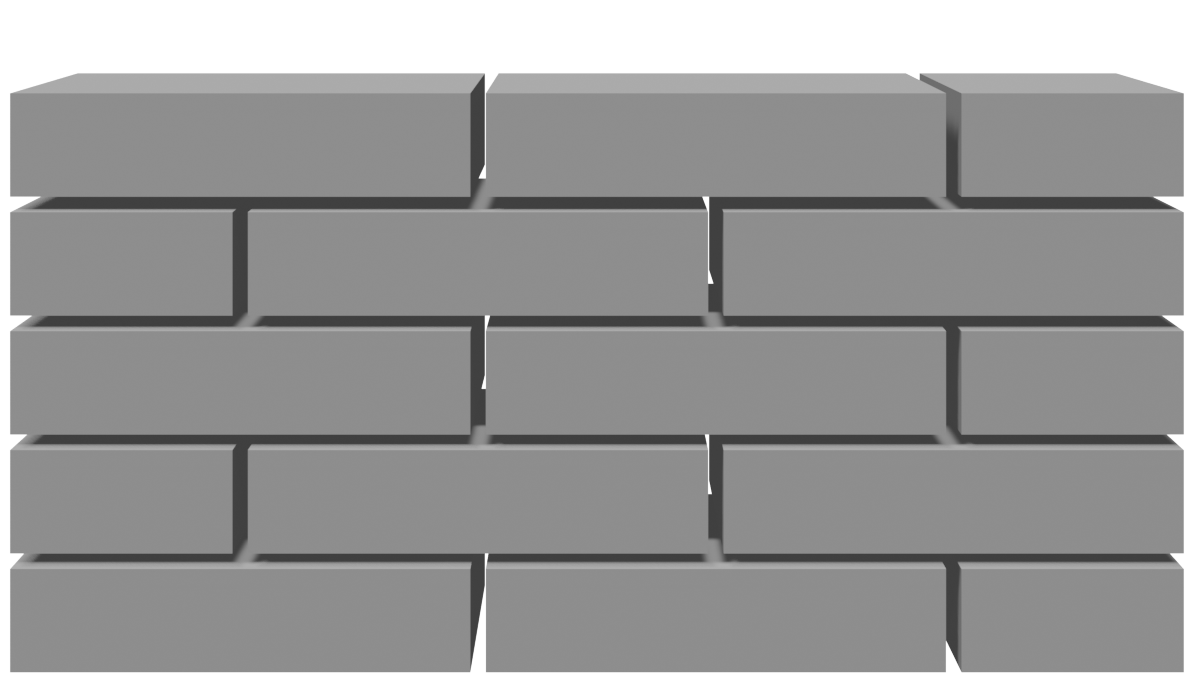
\includegraphics[width=\columnwidth]{fig/concept_wall_endings_1.png}
      \caption{Läuferverband.}\label{fig:concept:lauferverband_ending}
    \end{subfigure}
    \hfil
    \begin{subfigure}[b]{0.49\columnwidth}
      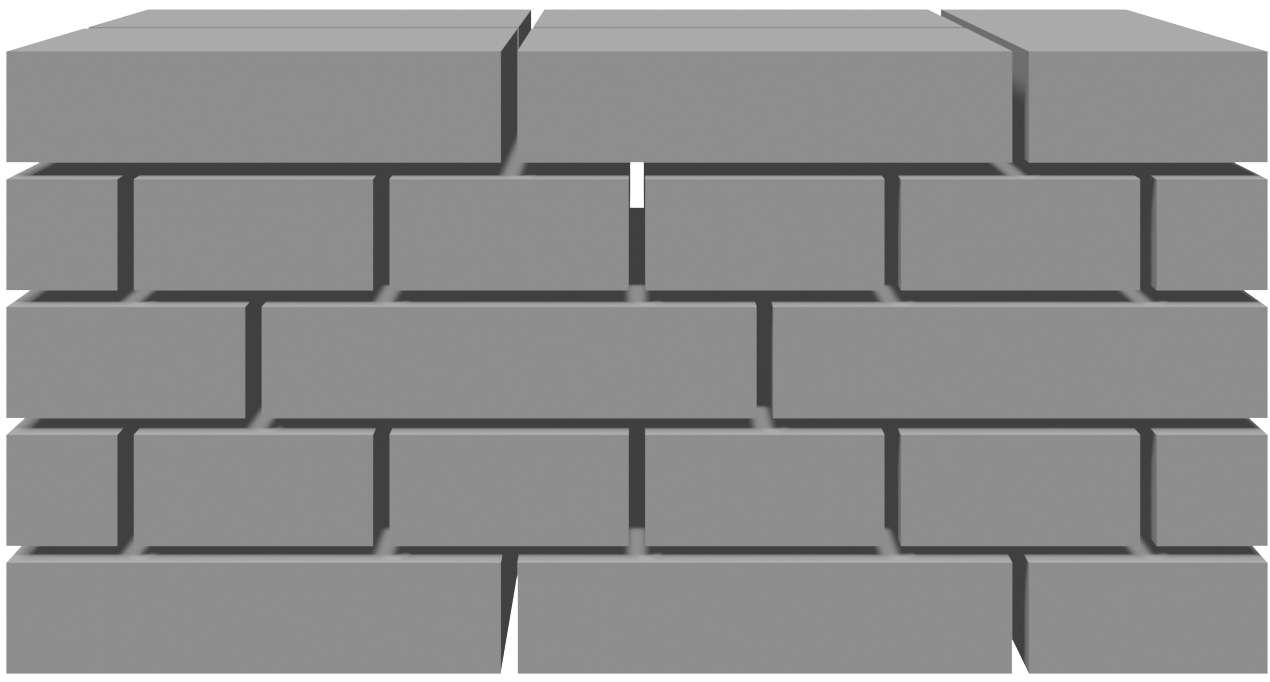
\includegraphics[width=\columnwidth]{fig/concept_wall_endings_2.png}
      \caption{Kreuzverband.}\label{fig:concept:kreuzverband_ending}
    \end{subfigure}
  \caption{Wandenden verschiedener Mauerwerksverbände.}
\end{figure}

In Abbildung~\ref{fig:concept:lauferverband_ending} werden für den Läuferverband Bausteine mit halber Modullänge und für den Kreuzverband in der Abbildung daneben zwei angepasste Versionen des Moduls benötigt:
Erneut ein Bausteinformat mit halber Modullänge um die Läuferverbandschichten des Kreuzverbands abzuschließen und ein Bausteinformat, dessen Länge sich aus der halben Modulbreite bildet und für den Abschluss der Kopfverbandschichten notwendig ist.
Aber nicht nur an Wandenden muss ein Mauerwerksverband mit einer geraden Kante abgeschlossen werden.
Auch an den zuvor angesprochen Öffnungen ist dies für die Schichten erforderlich, die durch die Öffnung geteilt werden.
Für den Fall, dass das vollständige Detailing eines Modells das Anpassen des gewünschten Moduls notwendig macht, muss diese Information neben den errechneten Transformationen der Bausteine ebenfalls in das Ergebnis integriert werden.
Somit erhält jeder Baustein aus diesem Grund zusätzlich eine Beschreibung über dessen Dimensionen.

\section{Wall Detailing}\label{concept:wall_detailing}
Als \glqq{}Wall Detailing\grqq{} (sprich das \glqq{}Detaillieren von Wänden\grqq{}) wird in dieser Arbeit der Vorgang bezeichnet, ein als geometrischer Körper definiertes Wandstück in konkretes Mauerwerk zu überführen.
Dieser Vorgang wendet die zuvor behandelten Konzepte an, um Lösungen für beliebig komplexe Gebäudemodelle zu errechnen.
Als Lösung sollen nur diejenigen Bausteinmengen gelten, die sämtliche von Wandstücken abgedeckten Bereiche lückenlos mit Bausteinen füllen, während gleichzeitig die gewünschten Mauerwerksverbände eingehalten werden.
Das nachfolgende schrittweise Verfahren weist aufgrund der ähnlichen Zielsetzung zwangsläufig Ähnlichkeiten zu dem von Usmanov et al.\ auf, das bereits in Kapitel~\ref{related:digital_plan_of_brickwork_layout} zusammengefasst wurde.

\begin{enumerate}
    \item Extrahieren relevanter Informationen wie Geometrie und Typ-Annotationen aus dem vorgegebenen Gebäudemodell. Dabei interessieren in erster Linie Wände und deren Öffnungen sowie gewünschte Module und Mauerwerksverbände (siehe Abschnitt~\ref{concept:mauerwerksverband}).
    \item Anwenden des vorgegebenen Moduls für jedes gefundene Wandstück. Das führt zu einer schichtweisen Repräsentation jedes Wandstücks. Dies erleichtert es später Operationen an und zwischen mehreren Wandstücken durchzuführen.
    \item Finden und Kombinieren von Wandstückverbänden nach Abschnitt~\ref{concept:combination_properties}.
    \item\label{concept:wall_detailing_tmp1} Finden und Lösen von anderen Beziehungen wie Ecken T- und X-Kreuzungen nach Abschnitt~\ref{concept:corner_etc_properties} (Finden) und Abschnitt~\ref{concept:solving_beziehungen} (Lösen).
    \item Schichtweises Anwenden der Öffnungen jedes Wandstücks. Dabei werden alle betroffenen Schichten in passender Weise geteilt und deren Länge reduziert.
    \item Schichtweises Anwenden der den Wandstücken zugewiesenen Mauerwerksverbände. Dazu gehören sowohl die besonderen Bereiche aus Punkt~\ref{concept:wall_detailing_tmp1}, als auch gerade Wandabschnitte und allein stehende Wandenden.
    \item\label{concept:wall_detailing_tmp2} Finden von (direkten) Nachbarschaftsbeziehungen zwischen Bausteinen.
    \item Konvertieren in das für die nachfolgende Bauplandeduktion notwendige Format.
\end{enumerate}

Das Ergebnis dieser Schritte ist eine Menge aus Bausteinen, nachfolgend auch als \textit{Bauplanentwurf} bezeichnet.
Durch die Berechnungen in Schritt~\ref{concept:wall_detailing_tmp2} werden bereits die grundlegendsten Beziehungen zwischen den Bausteinen hergestellt.
Eine Aussage darüber in welcher Reihenfolge die Bausteine gesetzt werden müssen, um das geplante Gebäude unter Berücksichtigung etwaiger physikalischer oder anderer Einschränkungen zu errichten, wird allerdings noch nicht getroffen.
Dazu müssen Schritt für Schritt Teilmengen aus der Gesamtmenge an Bausteinen extrahiert werden, die nur diejenigen Bausteine beinhalten, die in einer bestimmten Situation gelegt werden können.
Welche das sind, soll anhand vorgegebener Regeln ausgewertet werden können.
Diese Regeln können dafür verwendet werden bestimmte Voraussetzungen an einen Baustein zu setzen, um zum Beispiel das Ablegen eines Bausteins zu verhindern, unter dem sich weder fester Boden, noch ausreichend andere Bausteine befinden.
Denn setzt man einen Baustein mitten in der Luft ab, so fällt er in der echten Welt aufgrund der auf ihn einwirkenden Gravitation zu Boden.
Außerdem weisen unterschiedliche Bausteinarten und Umgebungen, in die man das Gebäude mithilfe des zuvor errechneten Bauplanentwurfs errichten möchte, womöglich unterschiedliche Einschränkungen auf.
So ist es notwendig je nach Situation voneinander abweichende Regelsets auf dem Bauplanentwurf anzuwenden zu können.
Die Möglichkeit der nachträglichen Definition dieser Regeln verhindert zusätzlich die Notwendigkeit den Bauplanentwurf für sich unterscheidende Situationen neu berechnen zu müssen.

\section{Regelbasierte Bauplandeduktion}\label{concept:regelbasierte_bauplandeduktion}
Ontologien bieten verschiedene Werkzeuge an, mithilfe derer sowohl streng definierte Objekttypen und deren Relationen zueinander modelliert, als auch konkrete Instanzen gruppiert und gefiltert werden können (siehe Kapitel~\ref{basics:ontologie}).
Da damit theoretisch sowohl Bausteindefinitionen und Instanzen, als auch Regeldefinitionen und konkrete Regeln formulierbar sind, ermöglicht dies ein flexibles Hinzufügen und Entfernen von Regeln und Bausteinen ohne dafür Programmcode schreiben zu müssen.
Durch geschicktes Aufstellen von Einschränkungen an die Bausteinklassen kann ein Reasoner dazu verwendet werden, ein den Regeln entsprechendes Subset derjenigen Bausteine zu bilden, die in der derzeitig in der Ontologie hinterlegten Ausgangssituation platzierbar sind.
Dies geschieht durch die Neuzuordnung einiger Bausteine zu einer speziell dafür definierten Klasse.
\begin{figure}[hbt]
  \centering
  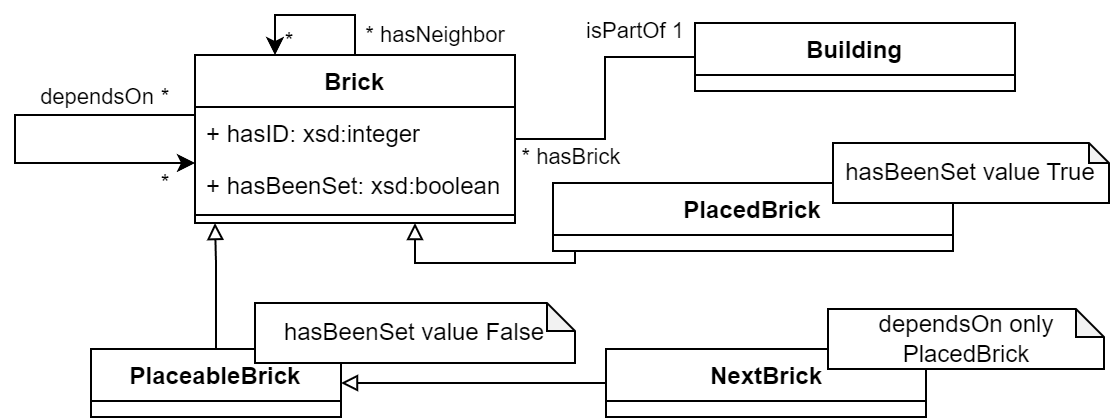
\includegraphics[width=0.8\columnwidth]{fig/klassendiagramm_ontologie_bricks.drawio.png}
  \caption{Klassendiagramm der Ontologie zur Bausteinbeschreibung.}\label{fig:concept:ontologie_diagramm_bricks}
\end{figure}
Notwendige Informationen für eine generische Ausgangsklasse zur Beschreibung von Bausteinen sind:
\begin{itemize}
  \item Eine eindeutige ID anhand derer für Bausteine aus der Ontologie die passenden Instanzen aus dem Programmcode identifiziert werden können.
  \item Nachbarschaftsrelationen zu anderen Bausteinen. 
  Da Bausteine sechs Seiten haben, an welchen andere Bausteine anliegen können, ist eine Unterscheidung zwischen den verschiedenen Nachbarschaftsarten (untere, obere, linke, rechte, vordere und hintere Nachbarn) möglich.
  \item Eine \textit{Abhängigkeits}-Eigenschaft zwischen Bausteinen, die angibt, an welchen Bausteinen jeder Baustein gebunden ist. 
  Diese Relation kann durch eine entsprechende Regel manipuliert werden und dadurch die Schlussfolgerungen eines Reasoners direkt beeinflussen. 
  Sie wird als Objekteigenschaft mit dem Namen \textit{dependsOn} realisiert, deren Wertebereich (Range) Individuen der Klasse Brick sind.
  \item Einen Indikator \textit{hasBeenSet} der angibt, ob der Baustein bereits gesetzt wurde oder nicht. 
  Darüber kann ein Reasoner verstehen, welche benachbarten Bausteine über die \textit{dependsOn}-Eigenschaft nicht mehr zu berücksichtigen sind.
\end{itemize}
Diese Klasse wird nachfolgend als \textit{Brick} bezeichnet und ist in Abbildung~\ref{fig:concept:ontologie_diagramm_bricks} dargestellt.
Um verschiedene Bauplanentwürfe gleichzeitig zu bearbeiten, kann eine Klasse \textit{Building} definiert werden, die alle Bausteine des dazugehörigen Bauplanentwurfs referenziert.
Eine Klasse \textit{Rule} stellt die Grundlage zur Regeldefinition dar.
Davon ausgehend können verschiedene Regelarten erstellt werden, die durch konkrete Individuen realisiert werden.
Ein Beispiel wären Regeln, die eine Kardinalität zu einer ebenfalls in der Regel festgelegten Daten- oder Objekteigenschaft der Ontologie vorgeben (für Informationen zu Eigenschaften im Kontext von Ontologien siehe Kapitel~\ref{basics:ontologie}).
Damit könnte etwa die Menge aller Nachbarn eines Bausteins auf exakt, minimal oder maximal eine bestimmte Anzahl beschränkt werden.
Eine weitere Art wären Regeln, die das Übernehmen einer bestimmten Eigenschaft auf alle über eine andere Eigenschaft assoziierten Bausteine voraussetzen.
So könnten zum Beispiel alle über die \textit{untere Nachbarn}-Eigenschaft verbundenen Bausteine eines konkreten Bausteins in dessen \textit{dependsOn}-Eigenschaft übernommen werden.
Notwendige Eigenschaften für diese Klasse sind:
\begin{itemize}
  \item Eine Assoziation auf eine Objekt- oder Dateneigenschaft der Ontologie, die angibt auf welche Eigenschaft die Regel Einfluss nimmt. 
  Dazu wurde die Eigenschaft \textit{holdPropertyByName} eingeführt. 
  Daraus werden die beiden Klassen \textit{DataPropertyHolder} und \textit{ObjectPropertyHolder} abgeleitet. 
  Alle Instanzen dieser Klassen haben den Namen einer Daten- oder Objekteigenschaft als String-Wert hinterlegt, denn Eigenschaften können im Kontext von Ontologien nicht direkt auf andere Eigenschaften verweisen.
  \item Eine Unterscheidung zwischen Regeln, die Kardinalitäten voraussetzen und jenen, die Eigenschaften übertragen. 
  Nachfolgend werden diese Klassen als \textit{CardinalityRule} und \textit{ApplyObjectPropertyRule} bezeichnet.
  \item Für Kardinalitäten-vorgebende Regeln existieren die Eigenschaften \textit{min}, \textit{max} und \textit{exactly}, welche auf einen Zahlenwert verweisen.
  \item Für Eigenschafts-übertragende Regeln existiert eine Eigenschaft, die ähnlich zu der aus dem obersten Punkt den Namen der \glqq{}Zieleigenschaft\grqq{} enthält.
\end{itemize}
\begin{figure}[htb]
  \centering
  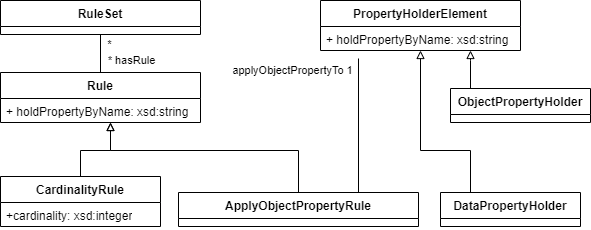
\includegraphics[width=0.7\columnwidth]{fig/klassendiagramm_ontologie_rules.drawio.png}
  \caption{Klassendiagramm der Ontologie zur Regelbeschreibung.}\label{fig:concept:ontologie_diagramm_rules}
\end{figure}

Eine Übersicht über diese Klassenstruktur ist in Abbildung~\ref{fig:concept:ontologie_diagramm_rules} zu sehen.
Um zwischen verschiedenen Situationen wechseln zu können, die manchmal die Anwendung mehrerer Regeln voraussetzen, wird die Klasse \textit{Ruleset} definiert, die lediglich auf beliebig viele Individuen der Rule-Klasse referenziert.

Mit diesem Aufbau wurde die Grundlage für einen Reasoner geschaffen, der die Individuen der Klasse Brick konkreteren Subklassen zuweist.
Eine Übersicht über diese Klassen ist ebenfalls in Abbildung~\ref{fig:concept:ontologie_diagramm_bricks} zu entnehmen.
Dabei stehen die Notizen, die an manche Klassen gehängt wurden, für die in der Ontologie hinterlegten Bedingungen, die für Individuen der jeweilige Klasse gelten müssen.
So lässt sich über die Werte in der \textit{hasBeenSet} Dateneigenschaft zwischen schon gesetzten und noch zu setzenden Brick-Individuen unterscheiden.
Diese Klassen werden als \textit{PlacedBrick} und \textit{PlaceableBrick} bezeichnet und sind zwangsläufig disjunkt.
Es können nur diejenigen Brick-Individuen, die ebenfalls der Klasse PlaceableBrick zugeordnet werden können, Teil des Subsets an Bausteinen sein, das in der derzeit gegeben Situation platziert werden kann.
Daraus lässt sich die erste Einschränkung für die als \textit{NextBrick} bezeichnete Klasse aufstellen:
Sie ist eine Subklasse der Klasse PlaceableBrick.
Die  \textit{dependsOn}-Eigenschaft der Klasse Brick wird nun zur Überprüfung der Legbarkeit eines Bausteins herangezogen.
Sind für einen PlaceableBrick nur PlacedBricks über diese Eigenschaft referenziert, so gilt dieser als derzeit ablegbar und wird ebenfalls Teil der Klasse NextBrick.
Insgesamt sieht die Klassenbeschreibung der Klasse NextBrick schließlich wie folgt aus:
\lstinline{PlaceableBrick and (dependsOn only PlacedBrick)}.
Zu beachten ist allerdings die \textit{Open World Assumption}, nach welcher sich Ontologien richten (siehe Kapitel~\ref{basics:ontologie}).
Darum ist es notwendig bei der Befüllung der Ontologie zusammen mit den im Bauplanentwurf errechneten Baustein-Instanzen explizite Einschränkungen vorzugeben.
Für jeden Baustein müssen alle konkreten Individuen definiert werden, die mit ihm über Eigenschaften verbunden sind.
Zusätzlich muss angegeben werden, dass diese Menge an Bausteinen auch tatsächlich die einzige unveränderbare Menge darstellt, die über sämtliche Eigenschaften damit verbunden sind.
Falls dies nicht vorgenommen wird, ist ein Reasoner nicht in der Lage ein PlaceableBrick-Individuum der Klasse NextBrick zuzuordnen, da es theoretisch sein könnte, dass ein anderer PlaceableBrick existiert, der der \textit{dependsOn}-Eigenschaft des Individuums zugeordnet ist.

Werden all die notwendigen Informationen zu den Bausteinen auf diese Weise und unter Einhaltung der definierten Regeln eines Regelsets in die Ontologie gespeist, kann durch Starten eines Reasoners das erste Subset aller platzierbaren Bausteine anhand der Zuordnung zu der Klasse NextBrick ausgelesen werden.
Nun kann daraus schrittweise ein Baustein gewählt und als platziert markiert werden, sodass mit erneuten Starten des Reasoners ein neues Set an Individuen der Klasse NextBrick errechnet wird, das zu der veränderten Situation und den vorgegebenen Regeln passt.
